% Copyright 2017 Remi Lehe
%
% This file is part of WarpX.
%
% License: BSD-3-Clause-LBNL


%%%%%%%%%%%%%%%%%%%%%%%%%%%%%%%%%%%
\section{Introduction}
%%%%%%%%%%%%%%%%%%%%%%%%%%%%%%%%%%%

\begin{figure}
%\begin{centering}
%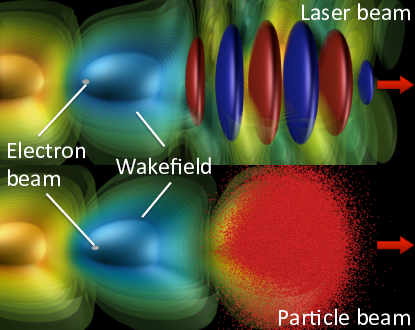
\includegraphics[trim={6cm 4cm 5cm 5cm},clip,scale=0.5]{Plasma_acceleration_sim.pdf}
%\immediate\write18{curl http://hifweb.lbl.gov/public/WarpX/test.png > Plasma_acceleration_sim.png}
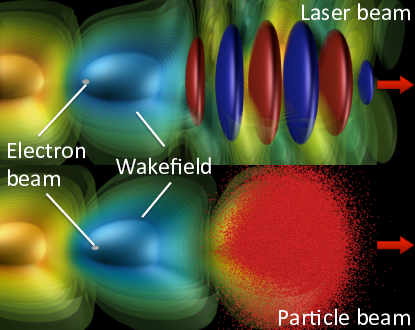
\includegraphics[scale=0.5]{Plasma_acceleration_sim.png}

%\par\end{centering}
\caption{\label{fig:Plasma_acceleration_sim} Plasma laser-driven (top) and charged-particles-driven (bottom) acceleration (rendering from 3-D Particle-In-Cell simulations). A laser beam (red and blue disks in top picture) or a charged particle beam (red dots in bottom picture) propagating (from left to right) through an under-dense plasma (not represented) displaces electrons, creating a plasma wakefield that supports very high electric fields (pale blue and yellow). These electric fields, which can be orders of magnitude larger than with conventional techniques, can be used to accelerate a short charged particle beam (white) to high-energy over a very short distance.}
\end{figure}

Computer simulations have had a profound impact on the design and understanding of past and present plasma acceleration experiments \cite{Tsungpop06,Geddesjp08,Geddesscidac09,Huangscidac09}, with
accurate modeling of wake formation, electron self-trapping and acceleration requiring fully kinetic methods (usually Particle-In-Cell) using large computational resources due to the wide range of space and time scales involved. Numerical modeling complements and guides the design and analysis of advanced accelerators, and can reduce development costs significantly. Despite the major recent experimental successes\cite{LeemansPRL2014,Blumenfeld2007,BulanovSV2014,Steinke2016}, the various advanced acceleration concepts need significant progress to fulfill their potential.  To this end, large-scale simulations will continue to be a key component toward reaching a detailed understanding of the complex interrelated physics phenomena at play.

For such simulations,
the most popular algorithm is the Particle-In-Cell (or PIC) technique,
which represents electromagnetic fields on a grid and particles by
a sample of macroparticles.
However, these simulations are extremely computationally intensive, due to the need to resolve the evolution of a driver (laser or particle beam) and an accelerated beam into a structure that is orders of magnitude longer and wider than the accelerated beam.
Various techniques or reduced models have been developed to allow multidimensional simulations at manageable computational costs: quasistatic approximation \cite{Sprangleprl90,Antonsenprl1992,Krallpre1993,Morapop1997,Quickpic},
ponderomotive guiding center (PGC) models \cite{Antonsenprl1992,Krallpre1993,Quickpic,Benedettiaac2010,Cowanjcp11}, simulation in an optimal Lorentz boosted frame \cite{Vayprl07,Bruhwileraac08,Vayscidac09,Vaypac09,Martinspac09,VayAAC2010,Martinsnaturephysics10,Martinspop10, Martinscpc10, Vayjcp2011,VayPOPL2011,Vaypop2011,Yu2016},
expanding the fields into a truncated series of azimuthal modes
\cite{godfrey1985iprop,LifschitzJCP2009,DavidsonJCP2015,Lehe2016,AndriyashPoP2016}, fluid approximation \cite{Krallpre1993,Shadwickpop09,Benedettiaac2010} and scaled parameters \cite{Cormieraac08,Geddespac09}.
